\documentclass[xetex,mathserif,serif]{beamer}
\usepackage{polyglossia}
\setdefaultlanguage[babelshorthands=true]{russian}
\usepackage{minted}
\usepackage{tabu}
\usepackage{moresize}
\usepackage{textpos}

\useoutertheme{infolines}

\usepackage{fontspec}
\setmainfont{FreeSans}
\newfontfamily{\russianfonttt}{FreeSans}

\definecolor{links}{HTML}{2A1B81}
\hypersetup{colorlinks,linkcolor=,urlcolor=links}

\tabulinesep=1.2mm

\title{GUI на WPF}
\subtitle{Часть 2}
\author[Юрий Литвинов]{Юрий Литвинов\\\small{\textcolor{gray}{y.litvinov@spbu.ru}}}
\date{23.11.2021}

\newcommand{\attribution}[1] {
\vspace{-5mm}\begin{flushright}\begin{scriptsize}\textcolor{gray}{\textcopyright\, #1}\end{scriptsize}\end{flushright}
}

\begin{document}

	\frame{\titlepage}

	\section{Команды}

	\begin{frame}
		\frametitle{Паттерн ``Команда''}
		\begin{center}
			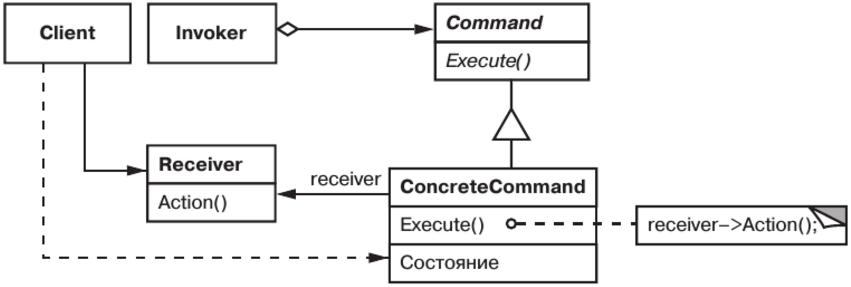
\includegraphics[width=0.9\textwidth]{command.png}
		\end{center}
	\end{frame}

	\begin{frame}
		\frametitle{Взаимодействие объектов}
		\begin{center}
			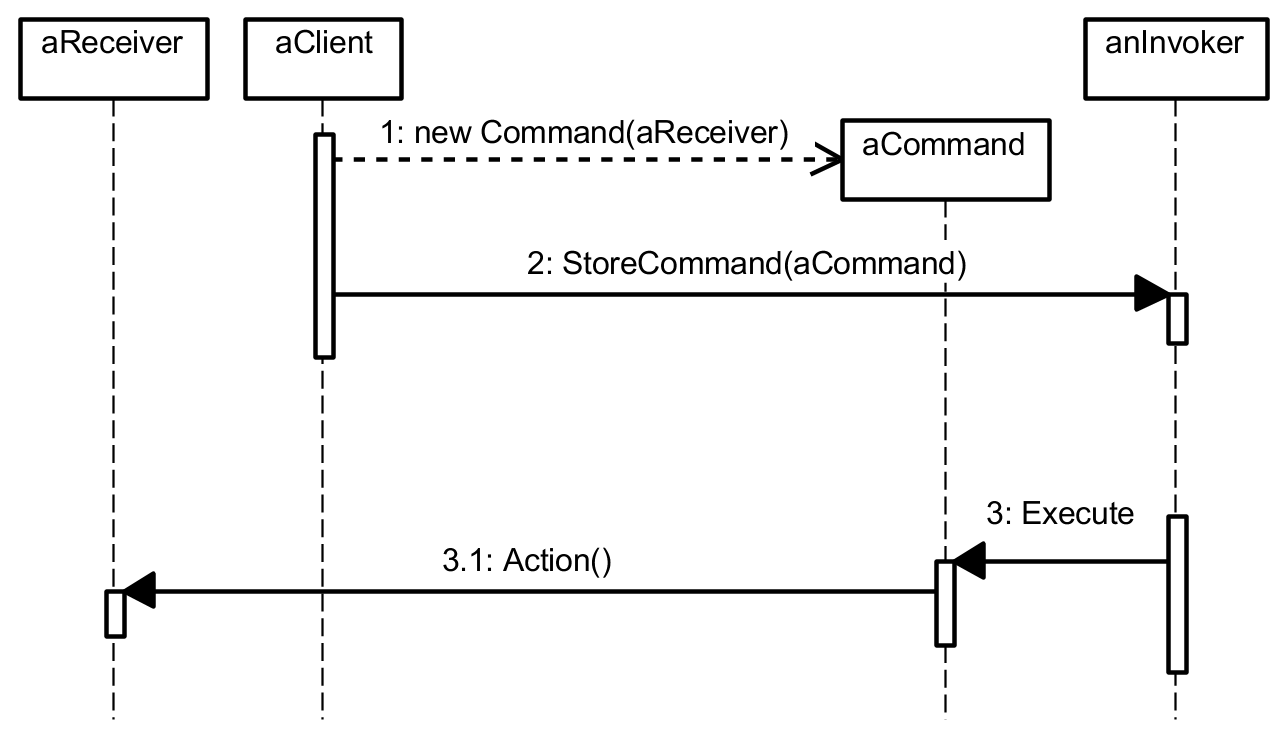
\includegraphics[width=0.9\textwidth]{commandSequence.png}
		\end{center}
	\end{frame}

	\begin{frame}[fragile]
		\frametitle{Команды}
		\begin{itemize}
			\item Интерфейс ICommand:
			\begin{itemize}
				\item Execute
				\item CanExecute
				\item CanExecuteChanged
			\end{itemize}
			\item Свойство Command
			\item Большой набор встроенных команд
			\item Класс CommandBinding
		\end{itemize}
		\begin{small}
			\begin{minted}{xml}
<Window.CommandBindings>
    <CommandBinding Command="Help"
        CanExecute="HelpCanExecute" Executed="HelpExecuted"/>
</Window.CommandBindings>
    ...
    <Button MinWidth="75" Margin="10" Command="Help" Content=
        "{Binding RelativeSource={RelativeSource Self}, Path=Command.Text}"/>
			\end{minted}
		\end{small}
	\end{frame}

	\section{Валидация}

	\begin{frame}[fragile]
		\frametitle{Валидация}
		\begin{scriptsize}
			\begin{minted}{csharp}
public class JpgValidationRule : ValidationRule
{
    public override ValidationResult Validate(object value, CultureInfo cultureInfo)
    {
        string filename = value.ToString();
        if (!File.Exists(filename))
            return new ValidationResult(false, "Value is not a valid file.");
        if (!filename.EndsWith(".jpg", StringComparison.InvariantCultureIgnoreCase))
            return new ValidationResult(false, "Value is not a .jpg file.");
        return new ValidationResult(true, null);
    }
}			\end{minted}
			\vspace{3mm}
			\begin{minted}{xml}
<TextBox>
    <TextBox.Text>
        <Binding …>
            <Binding.ValidationRules>
                <local:JpgValidationRule/>
            </Binding.ValidationRules>
        </Binding>
    </TextBox.Text>
</TextBox>
			\end{minted}
		\end{scriptsize}
	\end{frame}

	\section{Стили}

	\begin{frame}[fragile]
		\frametitle{Стили}
		\begin{scriptsize}
			\begin{minted}{xml}
<StackPanel Orientation="Horizontal">
    <StackPanel.Resources>
        <Style x:Key="buttonStyle">
            <Setter Property="Button.FontSize" Value="22"/>
            <Setter Property="Button.Background" Value="Purple"/>
            <Setter Property="Button.Foreground" Value="White"/>
            <Setter Property="Button.Height" Value="50"/>
            <Setter Property="Button.Width" Value="50"/>
            <Setter Property="Button.RenderTransformOrigin" Value=".5,.5"/>
            <Setter Property="Button.RenderTransform">
                <Setter.Value>
                    <RotateTransform Angle="10"/>
                </Setter.Value>
            </Setter>
        </Style>
    </StackPanel.Resources>
    <Button Style="{StaticResource buttonStyle}">1</Button>
    <Button Style="{StaticResource buttonStyle}">2</Button>
    <Button Style="{StaticResource buttonStyle}">3</Button>
</StackPanel> 
			\end{minted}
		\end{scriptsize}
		\begin{textblock}{3}(11,-11)
			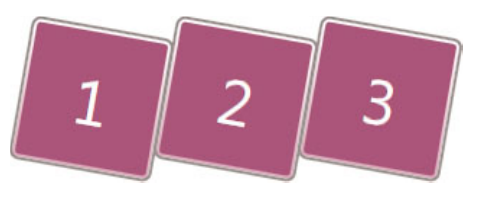
\includegraphics[width=\textwidth]{buttons.png}
		\end{textblock}
	\end{frame}

	\begin{frame}[fragile]
		\frametitle{Неявное применение стиля}
		\begin{scriptsize}
			\begin{minted}{xml}
<Application …>
    <Application.Resources>
        <Style TargetType="{x:Type Button}">
            <Setter Property="FontSize" Value="22"/>
            <Setter Property="Background" Value="Purple"/>
            <Setter Property="Foreground" Value="White"/>
            <Setter Property="Height" Value="50"/>
            <Setter Property="Width" Value="50"/>
            <Setter Property="RenderTransformOrigin" Value=".5,.5"/>
            <Setter Property="RenderTransform">
                <Setter.Value>
                    <RotateTransform Angle="10"/>
                </Setter.Value>
            </Setter>
        </Style>
    </Application.Resources>
</Application>
			\end{minted}
		\end{scriptsize}
	\end{frame}

	\begin{frame}[fragile]
		\frametitle{Триггеры}
		\begin{scriptsize}
			\begin{minted}{xml}
<Style x:Key="buttonStyle" TargetType="{x:Type Button}">
    <Style.Triggers>
        <Trigger Property="IsMouseOver" Value="True">
            <Setter Property="RenderTransform">
                <Setter.Value>
                    <RotateTransform Angle="10"/>
                </Setter.Value>
            </Setter>
            <Setter Property="Foreground" Value="Black"/>
        </Trigger>
    </Style.Triggers>
    <Setter Property="FontSize" Value="22"/>
    <Setter Property="Background" Value="Purple"/>
    <Setter Property="Foreground" Value="White"/>
    <Setter Property="Height" Value="50"/>
    <Setter Property="Width" Value="50"/>
    <Setter Property="RenderTransformOrigin" Value=".5,.5"/>
</Style>
			\end{minted}
		\end{scriptsize}
		\begin{textblock}{3}(11,-11)
			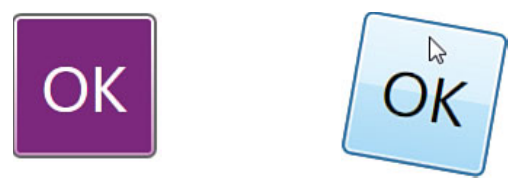
\includegraphics[width=\textwidth]{triggeredButtons.png}
		\end{textblock}
	\end{frame}

	\begin{frame}[fragile]
		\frametitle{Триггеры на значения свойств}
		\framesubtitle{Data Triggers}
		\begin{scriptsize}
			\begin{minted}{xml}
<StackPanel Width="200">
    <StackPanel.Resources>
        <Style TargetType="{x:Type TextBox}">
            <Style.Triggers>
                <DataTrigger
                    Binding="{Binding RelativeSource={RelativeSource Self}, Path=Text}"
                    Value="disabled">
                    <Setter Property="IsEnabled" Value="False"/>
                </DataTrigger>
            </Style.Triggers>
            <Setter Property="Background"
                Value="{Binding RelativeSource={RelativeSource Self}, Path=Text}"/>
        </Style>
    </StackPanel.Resources>
    <TextBox Margin="3"/>
</StackPanel>
			\end{minted}
		\end{scriptsize}
		\begin{textblock}{4}(11,-11)
			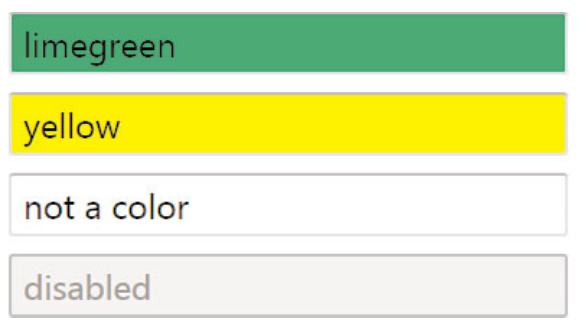
\includegraphics[width=\textwidth]{triggeredTextBoxes.png}
		\end{textblock}
	\end{frame}

	\section{Шаблоны}

	\begin{frame}[fragile]
		\frametitle{Шаблоны}
		\framesubtitle{Templates}
		\begin{ssmall}
			\begin{minted}{xml}
<Grid>
    <Grid.Resources>
        <ControlTemplate x:Key="buttonTemplate">
            <Grid>
                <Ellipse Width="100" Height="100">
                    <Ellipse.Fill>
                        <LinearGradientBrush StartPoint="0,0" EndPoint="0,1">
                            <GradientStop Offset="0" Color="Blue"/>
                            <GradientStop Offset="1" Color="Red"/>
                        </LinearGradientBrush>
                    </Ellipse.Fill>
                </Ellipse>
                <Ellipse Width="80" Height="80">
                    <Ellipse.Fill>
                        <LinearGradientBrush StartPoint="0,0" EndPoint="0,1">
                            <GradientStop Offset="0" Color="White"/>
                            <GradientStop Offset="1" Color="Transparent"/>
                        </LinearGradientBrush>
                    </Ellipse.Fill>
                </Ellipse>
            </Grid>
        </ControlTemplate>
    </Grid.Resources>
    <Button Template="{StaticResource buttonTemplate}">OK</Button>
</Grid>
			\end{minted}
		\end{ssmall}
		\begin{textblock}{2}(11,-11)
			
\includegraphics[width=\textwidth]{templatedButton.png}
		\end{textblock}
	\end{frame}

	\begin{frame}[fragile]
		\frametitle{Сохранение свойств элемента}
		\begin{scriptsize}
			\begin{minted}{xml}
<Viewbox>
    <ContentControl Margin="20" Content="{TemplateBinding Content}"/>
</Viewbox>
...
<LinearGradientBrush StartPoint="0,0" EndPoint="0,1">
    <GradientStop Offset="0"
        Color="{Binding RelativeSource={RelativeSource TemplatedParent},
        Path=Background.Color}"/>
    <GradientStop Offset="1" Color="Red"/>
</LinearGradientBrush>
			\end{minted}
		\end{scriptsize}
	\end{frame}

	\section{Ресурсы}

	\begin{frame}[fragile]
		\frametitle{Ресурсы}
		\begin{scriptsize}
			\begin{minted}{xml}
<Window ...>
    <Window.Resources>
        <SolidColorBrush x:Key="backgroundBrush">Yellow</SolidColorBrush>
        <SolidColorBrush x:Key="borderBrush">Red</SolidColorBrush>
    </Window.Resources>
    <Window.Background>
        <StaticResource ResourceKey="backgroundBrush"/>
    </Window.Background>
    <DockPanel>
        <StackPanel DockPanel.Dock="Bottom" Orientation="Horizontal"
            HorizontalAlignment="Center">
        <Button Background="{StaticResource backgroundBrush}"
            BorderBrush="{StaticResource borderBrush}" Margin="5">
            <Image Height="21" Source="zoom.gif"/>
        </Button>
    </DockPanel>
</Window>
			\end{minted}
		\end{scriptsize}
	\end{frame}

	\section{Задача}

	\begin{frame}
		\frametitle{Задача}
		\framesubtitle{GUI для клиента VK}
		\begin{itemize}
			\item Поле для ввода имени или id пользователя
			\item Поля, куда выводится имя/фамилия пользователя, полученные из VK
			\item Бонусное задание: Список, куда выводятся имена/фамилии из списка контактов пользователя
			\begin{itemize}
				\item Супербонусное задание: показывать статус (онлайн/оффлайн)
			\end{itemize}
			\item Кнопка ``Получить'', которая запускает процесс общения с сервером
			\begin{itemize}
				\item Бонусное задание: показывать данные по мере получения
			\end{itemize}
			\item Использовать паттерн MVVM и Command
		\end{itemize}
	\end{frame}

	\begin{frame}[fragile]
		\frametitle{Grid Layout}
		\begin{minted}{xml}
<Grid x:Name="mainGrid">
    <Grid.ColumnDefinitions>
        <ColumnDefinition Width="300"/>
        <ColumnDefinition Width="300"/>
    </Grid.ColumnDefinitions>
    <Grid.RowDefinitions>
        <RowDefinition Height="200"/>
    </Grid.RowDefinitions>

    <TextBox Grid.Row="0" Grid.Column="0" Margin="40, 5"/>
    <Button Grid.Row="0" Grid.Column="1" />
</Grid>
		\end{minted}
	\end{frame}

\end{document}
